
\begin{abstract}

The idea of Media-based Modulation (MBM), introduced in \cite{c0,isit2014}, is based on embedding information in the variations of the transmission media (channel state). This is in contrast to legacy wireless systems where data is embedded in a Radio Frequency (RF) source prior to the transmit antenna. MBM offers several advantages vs. legacy systems, including  ``additivity of information over multiple receive antennas'', and ``inherent diversity over a static fading channel''. MBM is particularly suitable for transmitting high data rates using a single transmit and multiple receive antennas (Single Input-Multiple Output Media-Based Modulation, or SIMO-MBM). However, complexity issues limit the amount of data that can be embedded in the channel state using a single transmit unit.  To address this shortcoming, the current article introduces the idea of Layered Multiple Input-Multiple Output Media-Based Modulation (LMIMO-MBM). LMIMO-MBM enables forming a high-rate constellation as superposition of constituent vectors due to separate transmit units.  Relying on such a layered structure, LMIMO-MBM can significantly reduce both hardware and algorithmic complexities, as well as the training overhead, vs. SIMO-MBM.  Exploiting the layered constellation structure, a fast iterative algorithm is proposed for signal detection, and a practical (small size and low complexity) RF  configuration is presented for embedding information in the channel state. Simulation results show excellent performance in terms of Symbol Error  Rate (SER) vs. Signal-to-Noise Ratio (SNR). For example, a $4\times 16$ LMIMO-MBM is capable of transmitting $32$ bits of information per (complex) channel-use, with SER~$\simeq 10^{-5}$ at $E_b/N_0\simeq -3.5$dB (or SER~$\simeq 10^{-4}$ at  $E_b/N_0=-4.5$dB). This performance is achieved using a single transmission (no extension in time/frequency), and without adding any redundancy for  Forward-Error-Correction (FEC).  As another example, a $2\times 8$ LMIMO-MBM is capable of transmitting 16 bits of information per (complex) channel-use, with SER~$\simeq 10^{-4}$ at $E_b/N_0\simeq 0.5$dB (or SER~$\simeq 10^{-3}$ at $E_b/N_0\simeq -0.8$dB).   This means, in addition to its excellent SER vs. energy/rate performance, MBM relaxes the need for complex FEC structures used in legacy wireless systems, and thereby minimizes the transmission delay. Overall, LMIMO-MBM provides a  promising alternative to MIMO and Massive MIMO for the realization of 5G wireless networks.


\end{abstract}

\section{Introduction}
Reference~\cite{c0} shows that embedding part or all of the
information in the (intentional) variations of the
transmission media (end-to-end channel) can offer
significant performance gains vs. traditional Single-Input Single-Output (SISO), Single-Input Multiple-Output (SIMO)
and Multiple-Input Multiple-Output (MIMO) systems. This method, coined in \cite{c0} as Media-Based Modulation (MBM), is in contrast with traditional wireless
systems where data is embedded in the
variations of an RF source (prior to the transmit antenna) to propagate via a fixed wireless channel (media) to the destination. In distinction to MBM, legacy modulation schemes are called Source-Based Modulation (SBM) hereafter. In particular, using capacity arguments, reference \cite{c0} shows that by using a single transmit antenna and a single or multiple receive antennas; MBM can significantly outperform SBM.

Following~\cite{c0}, reference \cite{isit2014}
proves that, a $1 \times K$ MBM over a
static multi-path channel asymptotically achieves the capacity
of $K$ parallel Additive White Gaussian Noise (AWGN) channels, where for each unit of energy
over the single transmit antenna, the effective energy for each
of the $K$ AWGN channels is the statistical average of channel
fading. In addition, the rate of convergence is computed. It is shown that significant gains
can be realized even in a SISO-MBM setup. An example
for the practical realization of the system using RF mirrors, accompanied with realistic RF and ray tracing simulations, are presented. Issues of equalization and selection
gain are also briefly discussed.

The idea of embedding information in the state of  a communications channel is not new. Mach–Zehnder modulators, widely used for signaling over fiber, modify the light beam after leaving the laser. However, due to the lack of multi-path in single mode fibers, the advantages due to SIMO-MBM and MIMO-MBM, realized in the context of wireless, do not apply. 

In distant relationship to MBM, there have been some recent works on embedding data in antenna beam-patterns. Note that unlike MBM, none of these works can realize advantages due to embedding information in the channel state. Most notably, these advantages, reported for the first time in~\cite{c0, isit2014}, include ``additivity of information over multiple receive antennas'' and ``inherent diversity without sacrificing transmission rate".

In \cite{c1} and \cite{c2}, data is embedded in two orthogonal antenna beam-patterns, which  can transmit a binary signal set. Although use of orthogonal basis is common in various formulations involving communications systems, it usually does not bring any benefits on its own, it just simplifies problem formulation and signal detection by keeping the noise projections uncorrelated. This means there are no clear advantages in designing the RF front-end to support orthogonal patterns as used in \cite{c1,c2}. The motivation in \cite{c1,c2} is to reduce the number of transmit chains and no other benefits are discussed. 

Bains~\cite{c3} discusses using parasitic elements for data modulation, and shows limited energy saving, which again is due to the effect of classical RF beam-forming. 

Spatial Modulation (SM)~\cite{c4-new} uses multiple transmit antennas with a single RF chain, where a single transmit antenna is selected according to the input data (the rest of the data modulates the signal transmitted through the selected antenna). SM is in essence a diagonal space-time code, where the trade-off between diversity and multiplexing gain has been in favor of the latter. A shortcoming of SM is that the rate due to the spatial portion increases with $\log_2$ of the number of antennas, while in MBM, it increases linearly with the number of RF mirrors (on-off RF mirrors are introduced in~\cite{isit2014} as means of embedding binary data in the channel state). In SM, antennas should be sufficiently separated to have independent fading, while in MBM, RF mirrors are placed side by side (in general, in MBM, the limit on the physical antenna separation is non-existent). The switches used in SM are high power, which means expensive/slow, or each antenna needs a separate Power Amplifier (PA) with switches placed before PAs. The switches used for RF mirrors in MBM are cheap, low power and fast.

The use of tunable parasitic elements external to the antenna(s) for the purpose of RF beam-forming is well established. However, the objective in traditional RF beam-forming is “to focus/steer” the energy beam, which does not realize the advantages of MBM (where data is modulated by tuning external parasitic elements).

The advantages of MBM, which are discussed in details in \cite{c0, isit2014}, are briefly explained next.
\begin{itemize}
\item Using MBM, it is possible to increase the number of constellation points without increasing transmit energy, while in legacy wireless systems, an increase in constellation size is accompanied with an exponential increase in constellation energy.
\item MBM offers an inherent diversity in dealing with static fading. Since constellation points in MBM correspond to different channel realizations, the spacing among points is formed using different channel gains. Hence, both good (high gain) and bad (low gain) channel conditions contribute towards forming the required spacing among constellation points. In other words, low channel gains result in constellation points closer to the origin, while high channel gains result in constellation points further away from the origin. As a result, constellation points are spread across the available transmission space. This feature is analogues to traditional modulation constructions, such as Quadrature Amplitude Modulation (QAM), which include constellation points over different energy shells distributed in the constellation space. This includes points near the origin (of low energy values) and far away from the origin (of high energy values), all contributing to the constellation cardinality and spacing. This feature of MBM removes the bottleneck of deep fades in static fading channels without compromising the rate. This is unlike traditional MIMO setups, where an increase in the diversity order is accompanied by a decrease in rate (multiplexing gain). In addition, a desirable feature of MBM is that the constellation points are spread across the signal space following a Gaussian distribution (due to Raleigh fading), which is in agreement with Gaussian random coding requirements. Relying on this feature, our earlier work reported in \cite{isit2014} shows that a $1 \times K$ MBM over a static multi-path fading channel asymptotically achieves the capacity of $K$ parallel AWGN channels, where for each unit of energy over the single transmit antenna, the effective energy for each of the $K$ AWGN channels is the statistical average of the channel fading. It was shown that significant gains can be realized even in a SISO-MBM setup due to inherent diversity \cite{c0}.

\item In $1 \times K$ SIMO-MBM, due to the independence of channel gains to different receive antennas, the received signal constellation spans all the $Q = 2 \times K$ receive dimensions. Therefore, MBM benefits from larger spacing among constellation points in case of using multiple receive antennas. This is analogous to additivity of information over multiple receive antennas~\cite{c0}. This is in contrast to SIMO-SBM where the received signal spans a single complex dimension, and consequently, only SNR gains can be achieved through techniques such as maximum ratio combining (without increasing the effective signal space dimensionality).
\item Another benefit of SIMO-MBM is the ``$K$ times energy harvesting'' which means, assuming $K$ receive antennas and a fading with statistical average gain of one, the average received signal energy is $ K$ times the transmit energy.

\end{itemize}

Some complexity issues arise when only a single RF transmit unit is used to realize the advantages of MBM at high data rates. Next section discusses the underlying practical issues, and present methods to address them.

\subsection{Limitations of SIMO-MBM in Transmitting High Date Rates}

Using a single transmit unit to embed all the information in the channel state will limit the amount of information that can be practically transmitted per channel-use. For example, let us assume we are interested to transmit $32$ bits of information per channel-use. The complexity in using a single RF transmit unit to encode all $32$ bits may be excessive. The reasons are:

\begin{itemize}
\item It is practically difficult to use $32$ RF mirrors in a single RF transmit unit (on-off RF mirrors are introduced in~\cite{isit2014} as means of embedding binary data in the channel state).

\item Training requires transmitting $2 ^ {32}$ test signals, which is resource intensive and is vulnerable to channel time variations.

\item Detection requires searching (minimum distance decoding) among $2 ^ {32}$ signal points, resulting in excessive algorithmic and storage complexities.

\item To deal with channel time variations, it is of interest to track the changes in the position of the constellation points in order to increase the minimum time interval between training phases. It is difficult to track $2 ^ {32}$ constellation points.

\end{itemize}


\subsection{Proposed Solution}
	
To address the above issues, this article proposes a new method to perturb the RF channel, resulting in a layered constellation structure.  Assume several separate transmitter units, each generating a set of received vectors (called ``constituent vectors" hereafter), operate at the same time. As a result, the received vector will be the sum of the constituent vectors corresponding to different transmit units. As the constituent vectors are random and independent from each other, the cardinality of the set of received vectors will be (with high probability) equal to the product of the cardinalities of the set of constituent vectors corresponding to different transmit units.  As a result, using $R_n$ RF mirrors at $N$ transmit units (each unit has a single radiating element) results in $2^ {N \times R_n}$ received vectors, capable of transmitting $R = N \times R_n$ bits of information per channel-use. Transmit units are arranged such that there is a negligible coupling among them. As a result, constellation points will be formed as the sum (superposition) of constituent vectors due to each transmit unit. To emphasize this superposition property, which forms the basis behind the complexity reduction, the proposed approach is called Layered MIMO-MBM, or LMIMO-MBM, hereafter. Benefits of this setup in reducing complexity are explained next.

\begin{itemize}

\item Number of RF mirrors used at individual transmit units is reduced by a factor of $N$.

\item Detection is performed using an iterative search algorithm. At each step, the proposed algorithm searches for the constituent vector contributed by each transmit unit (initializing the search by zero vectors) and continues iteratively. To improve the search result, one can start from multiple initial points (for example, corresponding to different permutations of transmit units).	

\item Training is simplified as it is composed of $N$ separate training tasks, each over a smaller set of alphabet size  $2^{R_n}$, as compared to training over $2 ^ {N \times R_n}$ elements.

\item Tracking is simplified as it is composed of $N$ separate tracking tasks, each over a smaller set of alphabet size $2^{R_n}$ elements, as compared to tracking $2 ^ {N \times R_n}$ elements. 

\end{itemize}

For example, to send $32$ bits of data per channel-use, one can use $4$ transmit units each modulating $8$ bits, which means only $8$ on-off RF mirrors are required in each transmit unit.  
Training/tracking is composed of $4$ separate tasks, each involving a small alphabet size of $2^8 = 256$ elements.

A disadvantage of the LMIMO-MBM method proposed in the current article  is that the received constellation vectors do not correspond to independent Gaussian vectors any longer (constellation vectors are summation of a smaller number of independent constituent vectors). This is in contrast with the requirement of Gaussian random coding over AWGN channels. However, the corresponding degradation in SNR performance is negligible. For example, Figure \ref{MIMOvsSIMO}  demonstrates this gap when minimum distance decoding is performed using exhaustive search. Since exhaustive search is not feasible for larger constellations, Figure \ref{algorithmPerformance} shows the performance of the proposed sub-optimal iterative decoder (to be explained later) for a constellation size of $2 ^ {32}$.


In the following, first the system model for SIMO-MBM and Layered MIMO-MBM are reviewed in section \ref{sec : System Model}. The benefits of using multiple transmit units in LMIMO-MBM are studied in more details in section \ref{sec : Benefits}. Subsequently in section \ref{sec: Detection Algorithm}, a sub-optimum iterative algorithm that enables fast detection in LMIMO-MBM setup is proposed. In section \ref{sec : Simulation Setup}, the LMIMO-MBM performance curve and the simulation setup, in which the error curves are obtained, is discussed. The issue of MBM potential bandwidth increase, due its time variant nature, is addressed in section \ref{sec : Pulse Shaping}. Finally, a practical (small size and low complexity) RF  configuration for embedding information in the channel state is presented in section \ref{RF Implementation}.

\section{System Model}
\label{sec : System Model}
\subsection{SIMO-MBM}
In a $ 1\times K $ SIMO-MBM system (as in Figure \ref{SIMO-MBM}), where there are $M$ messages to be sent, each message selects a channel realization $\rv{h}(m)$ with complex components $h(m), k = 1, ..., K $ and $m = 1, ..., M$. $\mathbb{E} {\mid\!h_k(m)\!\mid }^2 = 1$ where $\mathbb{E}$ denotes statistical averaging. Additional bits of information corresponding to SBM message $s$, can be transmitted, by directly modulating the RF signal. As an example, this can be done using RF phase shifter to modulate SBM information bits in the phase of the RF signal (e.g., selecting 0' or 180' phase shifts to generate $\mathbf{S}(s)$ for sending one additional bit). AWGN $\rv{z}$ has independent identically distributed (i.i.d.) components $z_k, \ k = 1, ..., K$, $ \mathbb{E}{\mid z_k \mid} ^2 = N_0$. Total transmission rate is equal to $R = \log_{2}{M}$ bits per channel-use. The receiver is trained to know $\rv{h}(m)$. This is done by sending a set of test signals for each possible channel realization (state) to measure received constellation $h_k(m), \ \forall m , \ \forall k$. For a Rayleigh fading channel,  $h_k(m)$ are i.i.d. complex Gaussian.

\begin{figure}[t]
\centering
%\hspace{-2mm}
\includegraphics[width = 12.5cm, height = 8.5cm, trim = 0cm 0cm 0cm 1cm ]{./fig/SIMOSystemModel_v4-AK}
\caption{SIMO-MBM block digram}
\label{SIMO-MBM}
\end{figure}

\begin{figure}[t]
\centering
%\hspace{-2mm}
\includegraphics[width = 12cm, height = 8.6cm]{./fig/MIMOSystemModel_v3-AK.pdf}
\caption{Layered MIMO-MBM (LMIMO-MBM) block digram}
\label{MIMO-MBM}
\end{figure}


\subsection{Layered MIMO-MBM (LMIMO-MBM)}

In a $ N\times K  $ MIMO-MBM system (as in Figure \ref{MIMO-MBM}), the ${M}$ messages to be sent are distributed among $ N $ transmit units, using vector $\rv{m}$ with components $m_1, ..., m_N$. Subsequently, each transmit unit selects its own channel realization vector $\rv{h}^n(m_n), n = 1, ..., N$,  according to $m_n$. These channel realization vectors, called constituent vectors hereafter, add to form the received constellation points $\mathbf{c}(\mathbf{m})$. Again, $\mathbb{E} {\mid {h}_k^n(m_n) \mid }^2 = 1, \ \forall{m}, \ \forall{n} \ \text{and} \ \forall{k} $. Similar to SIMO-MBM, each transmit unit can send optional SBM information bits. To attain this, transmit unit $n, n = 1, ..., N$, modulates its own RF signal based on the $n$th compnent of the information vector $\mathbf{s}$,  to generate RF modulated signal $\mathbf{S}_n(s_n), n = 1, ..., N$. Due to symmetry, distributing rate and power equally among individual transmit units results in the highest end to end mutual information. Throughout the paper, we assume power/rate is equal among transmit units. Consequently, the sets of LMIMO-MBM constituent vectors, corresponding to different transmit units, are of equal cardinalities, namely $ \sqrt[N]{M}=2^{R_m/N}=2^{R_n}$. For a Rayleigh fading channel, elements  of channel realization vectors $ {h}_k^n(m_n)$ are i.i.d. complex Gaussian. However, the received constellation vectors are no longer independent. Assuming unit transmit power for each transmit unit, we have

\begin{equation}
\label{eq:constellation}
\rv{c}(\mathbf{m}) = \sum_{n = 1} ^ { N} \rmat{h}^n(m_n),
\end{equation}
where $\rv{c}(\mathbf{m})$ is the received constellation point with $K$ complex dimensions. This means constellation points are formed as the superposition of constituent vectors due to each transmit unit. 

\section {Benefits of Using Multiple Transmit Units in LMIMO-MBM}
\label{sec : Benefits}
Using multiple transmit units simplifies receiver training and signal detection, specifically in transmitting large amounts of information per channel-use. Although MBM transmitter is oblivious to the details of the constellation structure, receiver training is required to convey the constellation structure to the receiver side. Training complexity grows linearly with the size of the constellation, making it an expensive task for constellations of large cardinalities. When using multiple transmit units in LMIMO-MBM, constellation set is formed by superposition of smaller sets of size $ \sqrt[N]{M}$. Therefore, one can measure ${h}_{k}^n(m_n) \ \forall n, \forall k \ \text{and} \ \forall m $, by sending pilot signals (using a single transmit unit at a time) and then constructing the entire constellation at the receive side by using superposition property (captured in equation \eqref{eq:constellation}). This means complexity of the receiver training will reduce from $\mathcal{O}(M)$ to  $\mathcal{O}(N\times \sqrt[N]{ M})$. Furthermore, there would be no need for huge memory to save all the constellation points $\rv{c}$, since on demand computation can take place, provided that constituent vectors $\rv{h}^n$ are known at the receive side.

Another benefit is the reduction in the complexity of signal detection by exploiting the structure of the constellation due to its layered construction. In this article, this benefit is realized using a (greedy/sub-optimum) iterative search algorithm, which searches among $\sqrt[N]{M}$ constituent vectors at each iteration.

In the proposed LMIMO-MBM, the dependency among constellation points results in a small decrease in the end-to-end mutual information, as compared to using random constellations, i.e., a constellation with i.i.d. Gaussian distribution for the components of the constellation points (resembling random Gaussian code-books). However, the performance degradation remains negligible (for example, see Figure \ref{MIMOvsSIMO}). 

Note that the performance shown in Figure \ref{MIMOvsSIMO} is over a single transmission, without using any FEC. It can be argued that in MBM, there is no need to use complex FEC structures which are typical in legacy wireless systems. However, the addition of FEC to MBM is straight-forward and can be realized with simple code structures with hard decision decoding, such as BCH (Bose-Chaudhuri-Hocquenghem) codes or RS (Reed-Solomon) codes. Moreover, signal detection can be performed with the lowest possible delay of a single symbol. These features of ``lowest possible decoding delay" and ``small error probability over a single time transmission" simplify the use of methods based on decision feedback, for example for the purpose of equalization and/or tracking the constellation structure in time.

\begin{figure}[t]
\centering
\hspace{1mm}
\includegraphics[width = 9.4cm, height = 7cm, trim = 6.5mm 0 -3mm 0 ]{./fig/MIMOvsSIMO2}
\caption{Performance of the 2$\times$8  LMIMO-MBM (2 RF mirrors are used in each transmit unit) vs. 1$\times$8 SIMO-MBM  (4 RF mirrors are used in a single transmit unit), $R = 16$ bits per channel-use for a single transmission in time (without any FEC). Note that at the cost of small degradation in performance and increasing the number of transmit units from one to two, the $2 \times 8$ LMIMO-MBM offers reduced complexity in each RF structure  and reduction in algorithmic complexity for training, detection and tracking.}
\label{MIMOvsSIMO}
\end{figure}


\section {Detection Algorithm}
\label{sec: Detection Algorithm}

In the presence of AWGN, for a given received signal $\rv{r} = \rv{c} + \rv{z} $, maximum likelihood detection for constellation point $ \rv{c}$ corresponds to $\hat{\rv{ c } }$, which is at minimum Euclidean distance to the received signal $\rv{r}$. A naive, but optimal solution for finding $\hat {\rv{c}}$ is exhaustive search among all constellation points. This so-called ``linear search'' is guaranteed to find the nearest point with a complexity of $\mathcal{O}(M)$. However, this operation can be very expensive for large signal sets. The problem of finding the nearest member (in our case, in Euclidean distance sense) of a set of predefined points to a query point, also known as Nearest Neighbor Search (NNS), has many applications, including in pattern recognition, statistical classification, computer vision, etc. Therefore, the NNS problem has been widely studied and many algorithms have been suggested in the literature. However, none of these  existing classes of algorithms appeared to be suitable for LMIMO-MBM setup due to the reasons explained next.

\subsection {A Review of Potentially Suitable Search Algorithms}
A general approach for reducing the complexity of a full search in NNS problem is based on preprocessing data points (in our case, constellation points) and storing them in a suitable data structure, such as k-d trees~\cite{kdtree1}. This provides a near optimal solution for cases of low dimensionality. However, the complexity of most these algorithms grow exponentially with the number of dimensions, which is the case when multiple receive antennas are used in MBM. This results in a search complexity comparable to that of the naive ``linear search''.
Furthermore, due to the nature of propagation media, channel realizations, and hence the constellation points, change in time. Therefore, a detection algorithm which relies on extensive preprocessing of the constellation points will not be favorable. Another approach to reduce the complexity is based on Triangle Inequality Elimination (TIE)~\cite{TIE1, TIE2, TIE3, TIE4}. In this class of methods, reference points are used and their distances to actual data points are precomputed and stored. In the search phase, the distances between the query and the reference points are calculated. Then, using the precomputed distances and a simple comparison, a large number of data points are eliminated. A drawback of this technique is its large memory requirement (larger than the constellation size itself) to store the precomputed distances, as well as the computational overhead due to the required preprocessing.

In the following, a fast greedy iterative algorithm, enabled by layered structure of the proposed MIMO-MBM, is used for sub-optimal minimum distance signal detection. Advantages of the proposed algorithm include:

\begin{itemize}

\item The complexity grows as $\mathcal{O}( \sqrt[N]{M})$ compared to $\mathcal{O}(M)$ in linear search.

\item The complexity grows linearly with the number of dimensions in contrast to the alternative search mechanisms known in the literature of NNS.

\item The algorithm does not require any storage space more than what is required to store channel realizations (constituent vectors) for the individual transmit units, which is of order $\mathcal{O}( N \times \sqrt[N]{M})$.

\item There is no need for preprocessing, in contrast to alternative search mechanisms known in the literature of NNS.

\end{itemize}

\subsection{MIMO-MBM  Greedy/Iterative Search Algorithm}

\textbf{Iterations}: Algorithm \ref{pseudocode} is the pseudocode for the proposed sub-optimum minimum distance detection in LMIMO-MBM. Each iteration is composed of $N$ greedy steps. At each step, the algorithm attempts to (successively) find the constituent vector corresponding to a single transmit unit. At step $i$, a potential solution $\hat{ \rv{c} } ^ {(i)}$, for the minimum distance vector to the query signal $\rv{r}$ is given as the current best solution. Suppose $\hat{ \rv{c} } ^ {(i)}$ is formed by superposition of constituent vectors $(\hat{\mathbf{h}}^1, ..., \hat{\mathbf{h}}^N)$. The algorithm compares the constituent vector corresponding to transmit unit $i$, which means $\hat{\mathbf{h}}^{i}$, with all other vectors in the set $\mathcal{H}^{i} = \{ \mathbf{h}^{i}(1), ..., \mathbf{h}^{i}(2^{R_n}) \}$ of constituent vectors corresponding  to transmit unit $i$. Subsequently $\hat{\mathbf{h}}^{i}$ is replaced with the vector $\tilde{\mathbf{h}}^{i}$ in $\mathcal{H}^{i} $ that results in a constellation point $\hat{ \rv{c} } ^ {(i+1)}$, which (among all choices available at this step) is the closest to the signal $\mathbf{r}$. Therefore, 

\begin{equation}
\tilde{\mathbf{h}}^{i} = \underset{\mathbf{h} \in  \mathcal{H}^{i}}{\text{argmin}} {\mid \rv{r} - (\hat{\rv{c} } ^ {(i)} - \hat{\mathbf{h}}^{i}+ \mathbf{h})\mid} _ 2
\label{neighbor_search}
\end{equation}

\begin{equation}
\hat{\rv{c} } ^ {(i+1)} = \hat{\rv{c} } ^ {(i)}- \hat{\mathbf{h}}^{i}+ \tilde{\mathbf{h}}^{i}
\end{equation}

 In other words, at each step, a search over constituent vectors corresponding to a single transmit unit is performed (based on the current knowledge of signals of the other transmit units). $\hat{\rv{c} } ^ {(N+1)}$ is passed to the next iteration as the current best candidate, i.e., closest to the query signal $\mathbf{r}$. Each iteration is composed of $N$ such steps, and in total $T$ iterations are performed before concluding the search. As can be seen in \eqref{neighbor_search}, there is no need to store all constellation points, since they can be computed on the fly using constituent vectors.

\textbf{Initialization}: At the first step of first iteration, there is no prior knowledge of any of the constituent vectors. Therefore, $\hat{\rv{c} } ^ {(1)}$ is initialized to a vector of all zero elements, which in fact is not a valid constellation point. At the end of the first iteration (i.e., after $N$ steps), $\hat{\mathbf{c}}^ {(N+1)}$ will be a valid constellation point.

\textbf{Improving the Search}: The algorithm in its simple form explained above can find the optimum solution in vast majority of cases. However, since we are dealing with very low Symbol Error Rate (SER) values, even a small number of errors due to the algorithmic failure (e.g. iterations end-up in a loop) can govern the performance and result in error floor. Simulation results show the decoded constellation point for a fixed received signal $\mathbf{r}$ may be different when different ordering of transmit units for (successive) decoding is considered. For that reason, multiple runs of the above algorithm corresponding to different permutations of transmit units is used to improve the search. Each of these runs correspond to one of $N!$ possible permutations of the sequence $(1, ..., N)$ as the order of the transmit units to be decoded.

The performance can be further improved by using multiple (i.e $P>1$) points for each of the runs. This means at step $i$, given $P$ best points as the current solution,  the algorithm replaces the $i$th constituent vector in each of these $P$ points with  constituent vectors in the set $\mathcal{H}^{i}$, and returns an improved $P$ best points (that are closest to vector $\mathbf{r}$) for the next step (or next iteration). Larger values for $P$ increases the chance of finding the nearest point to $\rv{r}$. 

\begin{figure}[t]
\centering
\hspace{-1cm}
\vspace{0cm}

{\includegraphics[height = 6.6cm, width = 9cm, trim = 6cm 9.6cm 6cm 10cm ]{./fig/algorithm_performance}}
\caption{Performance of 4$\times$16 MIMO-MBM for a single transmission (without any FEC), $R = 32$ bits per channel-use, detection is performed using Algorithm \ref{pseudocode} considering different permutations of transmit units with $ P = 128, T =2$.}
\label{algorithmPerformance}
\end{figure}

\begin{algorithm}[t]
%\begin{footnotesize}
\caption{Iterative detection algorithm}\label{pseudocode}
 Search for the nearest (Euclidean distance) constellation point to received signal $\rv{r}$ 
\begin{algorithmic}[1]
\Function{find} {$\rv{r}$}
\State $\hat{\rv{c} } ^ {(N+1)} = \mathbf{0}$
\For{$j = 1, ..., T$} \Comment{$j$ is the loop index for iterations}
\State $\hat{\rv{c} } ^ {(1)} = \hat{\rv{c} } ^ {(N+1)}$
\For{$i = 1, ..., N$} \Comment{$i$ is the loop index for steps}

\State $\tilde{\mathbf{h}}^{i} = \underset{\mathbf{h} \in  \mathcal{H}^{i}}{\text{argmin}} {\mid \rv{r} - (\hat{\rv{c} } ^ {(i)} - \hat{\mathbf{h}}^{i}+ \mathbf{h})\mid} _ 2$
\State $\hat{\rv{c} } ^ {(i+1)} = \hat{\rv{c} } ^ {(i)}- \hat{\mathbf{h}}^{i}+ \tilde{\mathbf{h}}^{i}$

\EndFor\label{tend}
\EndFor
\State \textbf{return}  $\hat{\rv{c} } ^ {(N+1)}$\Comment{nearest point}
\EndFunction

\end{algorithmic}
%\end{footnotesize}
\end{algorithm}

\section {Simulation Setup}
\label{sec : Simulation Setup}

For the simulation of the proposed LMIMO-MBM system, the constituent vectors corresponding to each transmit unit are generated with complex i.i.d. Gaussian random components of unit variance, and then their linear combination is used to form the constellation. The performance is averaged over many independent runs. $E_b$, energy per bit, is defined as the sum of signal energies of transmit units divided by the total number of bits per transmission, and $N_0$ is the AWGN spectral density at individual receive antennas. Therefore, 

\begin{equation}
\label{ebn0}
E_b/N_0 =\frac{NE}{RN_0},
\end{equation}
where $E$ is the signal energy corresponding to each transmit unit.


Figure \ref{algorithmPerformance} shows the SER performance for $ 4\times 16$ LMIMO-MBM, over a static Rayleigh fading channel with AWGN, transmitting $32$ bits of raw data per channel use. Detection is concluded after two iterations (over $4$ transmit units), using $P = 128$ candidate points and considering different permutations of transmit units.

\section{Application of Forward Error Correction Codes}


In the application of Forward Error Correction (FEC) to MBM, it is beneficial to consider coding schemes that operate on MBM symbols. It is straightforward to generalize known good binary codes such that the underlying parity equations operate on modulated symbols, and accordingly, the addition operations will be modulo the constellation size. As an example, a Single Parity Check Code, abbreviated as SPC hereafter, can be expressed as:


\begin{equation}
\sum_n BLABLA_i=0 mod THE SIZE (i guess it would be 2^R)
\end{equation}


It is straightforward to show that by applying such a coding scheme, the slope of the error rate vs. SNR will asymptotically increase by a factor of $d_{min}$, where $d_{min}$ is the minimum distance of the original binary code. This occurs as the spacing between pairs of points, namely $A-B$ for points $A$ and $B$, in MBM is a Gaussian random variable, and for three points $A,B,C$, $A-B$ is independent of $A-C$.
Consequently, application of FEC will realize an effect similar to ``diversity over time” with a diversity order determined by $d_{min}$. The corresponding compromise in effective rate is determined by the rate of the underlying binary
 code. Note that conventional binary codes are designed to achieve the best possible tradeoff between $d_{min}$ and effective rate, i.e., have a large $d_{min}$ for a given rate. As a result, by applying good known binary codes to MBM through generalization
 of parity equations mentioned above, the resulting error performance will enjoy the best achievable asymptotic slope.


Figure ?? shows this effect for an SPC with $(n,k,d)=(6,5,2)$.


Figure ?? shows the performance in the application of Reed-Solomon (RS) codes with symbols corresponding to MBM constellation points.


Note that, unlike random-like codes such as Turbo-code and Low Density Parity (LDPC) codes which typically suffer from error floor, the slope of the error curve in coded MBM will not change as SNR increases.


\begin{figure}[t]
\centering
%\hspace{-1cm}
\vspace{-1cm}

{\includegraphics[scale = 0.65,  trim = 3cm 5cm 3cm 5cm]{./fig/MBM_coded}}
\caption{Performance of 4$\times$16 MIMO-MBM with  FEC applied.}

\label{coded}
\end{figure}


\section {Pulse Shaping, Equalization and Decision Feedback at the Receiver}
\label{sec : Pulse Shaping}
MBM inherently corresponds to a linear time variant system. Unlike linear time invariant systems, which maintain the spectrum occupancy of the signal, a linear time variant system can potentially increase the bandwidth. The issue of increase in band-width can be tackled by using the combination of the two methods explained next.

\textbf{Pulse Shaping:} This corresponds to applying a pulse shaping filter at the transmitter in the time domain, such as raised cosine, to smoothen the transition between successive transmission pulses.


\textbf{Silent Transmissions:} This corresponds to inserting gaps of zero transmission (transmitter remains silent) between successive transmission pulses (see Figure \ref{pulse shaping}), and sampling at the receiver side corresponding to both on and off transmission intervals. Due to channel impulse response, the receiver will receive values even during the periods that the transmitter has remained silent. Receiver relies on all received values for signal detection. Note that impulse responses, corresponding to different channel states in MBM, are independent from each other. As a result, a longer channel impulse response increases the effective dimensionality of the receive signal space. For example, using $D = 2$ time slots in conjunction with $8$ receive antennas results in $16$ receive dimensions. Similarly, $D = 4$ time slots in conjunction with $4$ receive antennas, result in $16$ receive dimensions. Note that, if the length of the channel impulse response is larger than $D$, then there will be propagation from each pulse into its subsequent time intervals beyond the window of length $D$. Since we are dealing with very low SER values, the effect of this propagation beyond the window of length $D$ can be removed using decision feedback. This means, receiver can decide for the transmitted message (corresponding to a given constellation in time) and account for its propagation into the next set of values (by subtracting the effect of the propagated signal). This is performed prior to the decoding of the subsequent constellation symbols. Simulation results show that, even for $D = 2$ which is realizable in a channel with an impulse response of a length greater than or equal to two, using raised cosine pulse shaping, the out-of-band radiation is significantly below the levels allowed in current wireless standards. Note that using $D = 2$ allows for a bandwidth expansion by a factor of two, which is quite larger than the spectral expansion due to time varying nature of MBM. 

As a side benefit, increasing dimensionality of the received signal space through silent transmissions allows reducing the number of receive antennas proportionally.  


\begin{figure}[t]
\centering
\hspace{1cm}
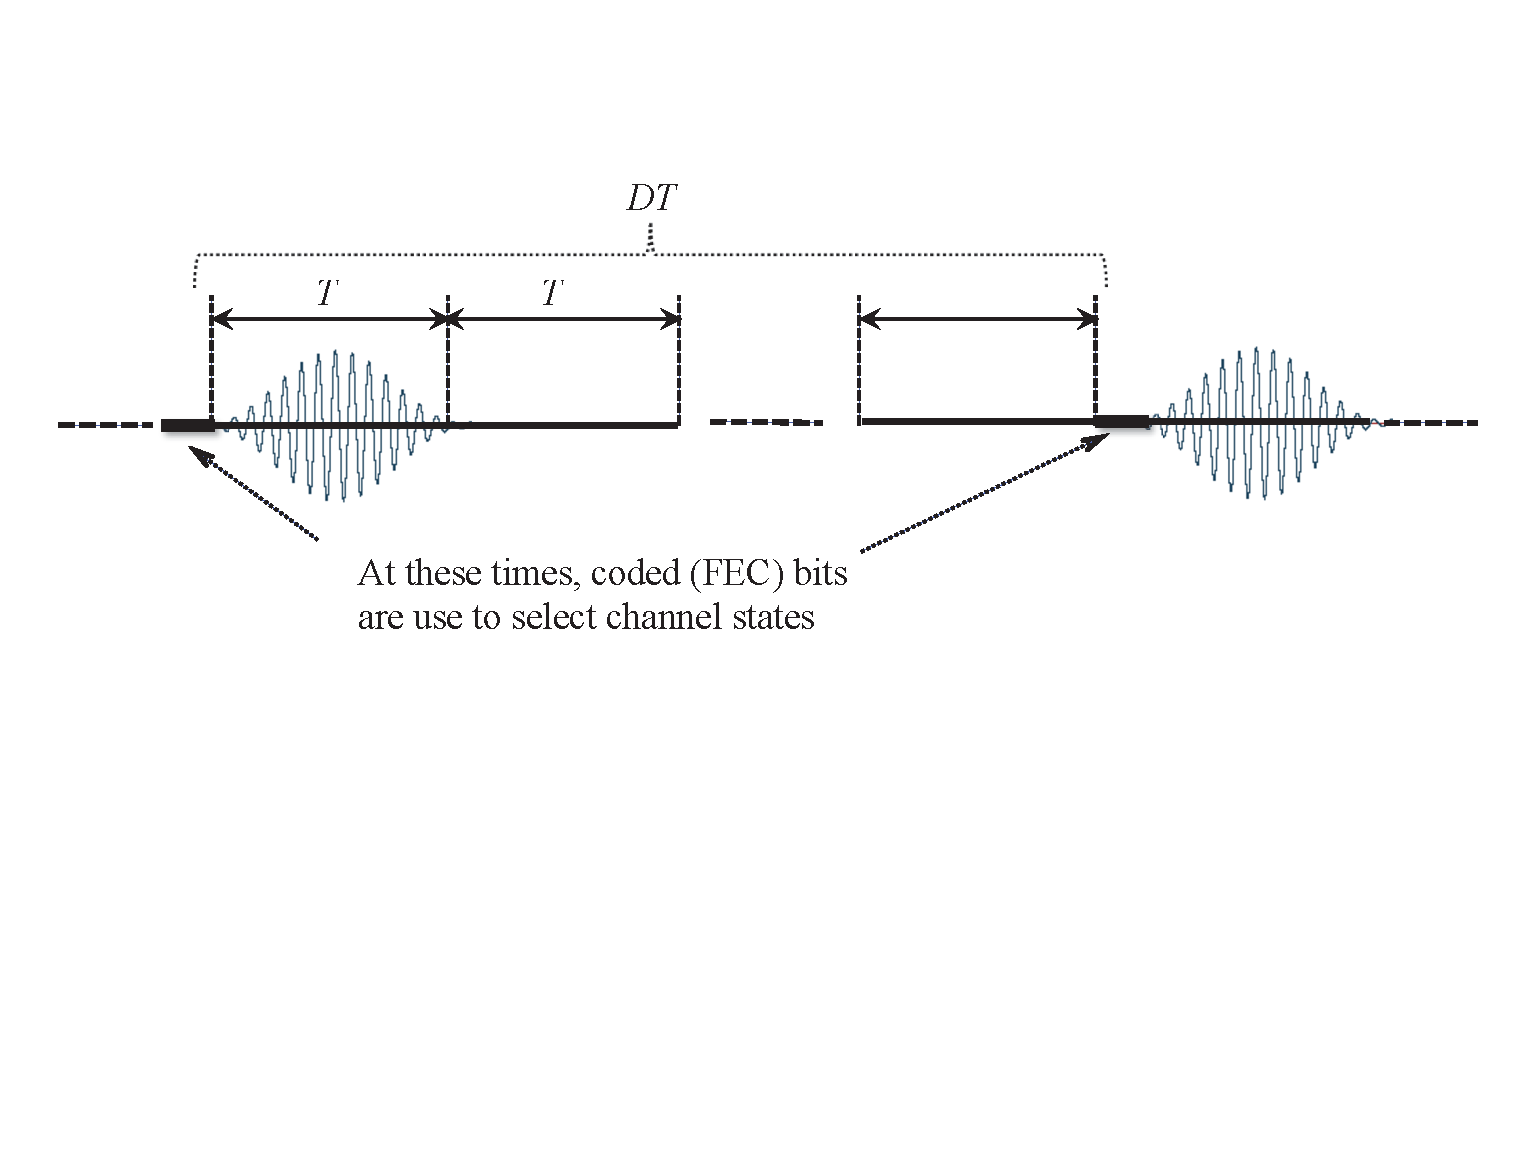
\includegraphics[height = 5cm, width = 9cm, trim = 0 8cm 0 0cm]{./fig/pulseShaping}
\caption{Pulse shaping in time}
\label{pulse shaping}
\end{figure}

\begin{figure}[t]
\centering
\hspace{1cm}
\vspace{0cm}
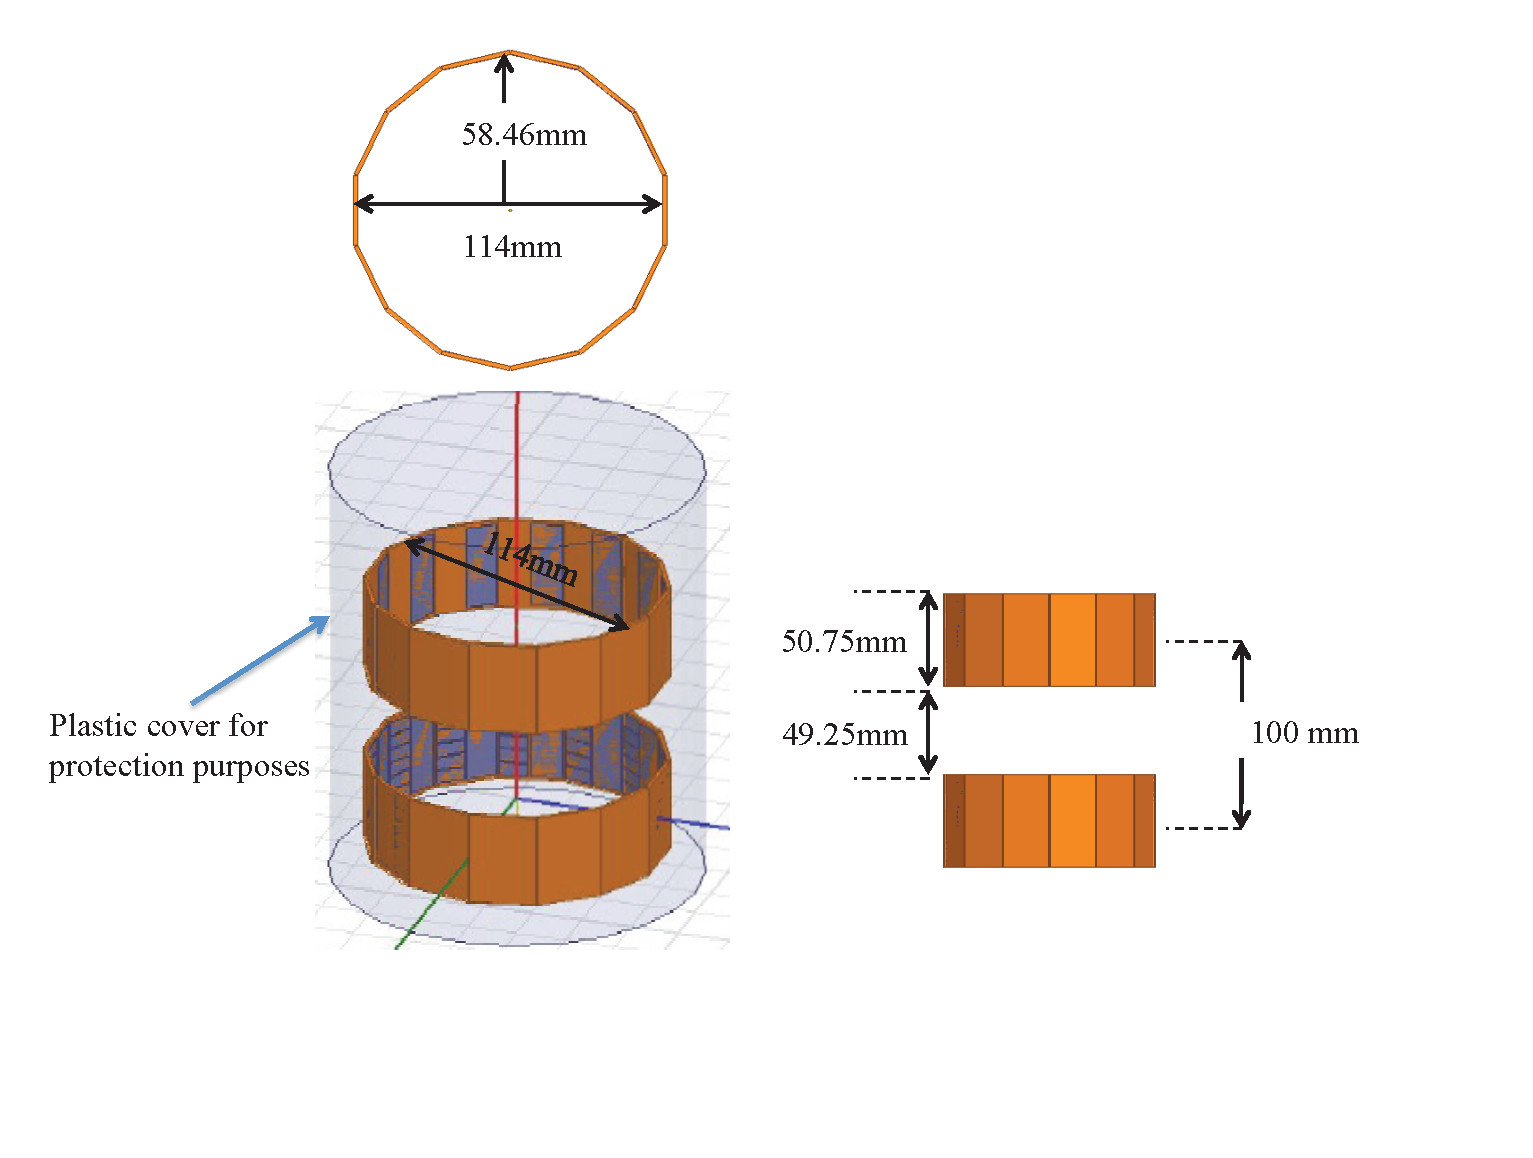
\includegraphics[width = 9cm, height = 5.5cm, trim = 0 2cm 1cm 1.2cm]{./fig/ParasiticAntenna1}
\caption{Two transmit unit stacked vertically. Note that more units can be stacked using a similar structure.}
\label{SingleUnit}
\end{figure}

\begin{figure}[t]
\hspace{3.7cm}
\vspace{0.5cm}
\includegraphics[ width = 11cm, height = 6cm, trim = 1cm 0 0 0cm]{./fig/ParasiticAntenna2}
\caption{Structure of a single RF mirror, all diodes are turned on and off (switched) simultaneously.}
\label{SinglePCB}
\end{figure}

\section{RF Implementation}
\label{RF Implementation}
Figure \ref{SingleUnit} shows 2 RF transmit units stacked uniformly along the $z$ direction. Vertical stacking of transmit units reduces the RF coupling among them. The gap between adjacent units is 100~mm. Simulation result (using High Frequency Structural Simulator, HFSS) shows that this spacing results in about $-25$~dB coupling at 5.8~GHz. Each unit is formed using 14~RF mirrors. Printed Circuit Boards (PCBs) have a thickness of 60~mil. The height and diameter of the units are 50.75~mm and 116.92~mm, respectively.
Each PCB consists of two main parts with a spacing of 0.82~mm: (i) a monolithic rectangular copper part of size 46.75~mm $\times$ 12.5~mm, and (ii) seven rectangular patches with a length of 7.25~mm and width of 11.20~mm.The dimensions of patches are optimized at 5.8~GHz using HFSS to achieve high transmission efficiency ($S_{ii}<-15dB$) and low coupling ($S_{ij}<-25dB$).
Each two adjacent patches can be connected or disconnected using a diode (as an RF switch). In each RF mirror, all diodes are turned on or off (switched) simultaneously. The gap between two adjacent patches is 0.65~mm. A dipole antenna is placed at the center of each unit as the radiating element. Each RF mirror will be transparent to, or will reflect the incident wave, if its diodes are open or short, respectively. Each RF mirror in each transmit unit can be switched independently. Using $14$ mirrors results in $2^{14}$ channel states, where a subset of a smaller size, say 256, is used to transmit individual constituent vectors in the proposed LMIMO-MBM structure.

To avoid using multiple transmit chains, a single transmit chain, i.e., single base-band, single RF modulator, single Power Amplifier (PA), can be used as shown in Figure~\ref{single_rf_chain}. The RF phase shifters can be used for sending additonal (source-based modulated) data. For example, one can select 0' or 180' phase shifts according to one additional bit of information (per transmit unit), or  0',90',180',270' phase shifts according to two additional bits of information (per transmit unit). The RF phase shifters can also facilitate training as will be explained next.

In the training phase, to train for each transmit antenna, one possible option is to bypass (disable)
the remaining antennas using RF switches (shown as optional components in Figure~\ref{single_rf_chain}).
Another option is to train for each antenna when the other antennas are configured to transmit a default signal (e.g., transmit the constituent vector indexed by zero). In this case, the receiver will be first trained to learn the received vector corresponding to the tranmission of the default constituent vector for each transmit unit. To train the receiver for the default constituent vectors, one can use the 0',180' phase shifts to realize $\pm 1$ towards forming of a Hadamard basis over transmit units. As a result, there is no need for RF switches in Figure~\ref{single_rf_chain}, and trainings for default constituent vectors can be realized using phase shifters with at least two selectable phase values, 0' and 180', to multiply the signal from each transmit antenna by $+1$ or $-1$, respectively. In this case, the receiver will be able to invert the Hadamard basis and extract the response corresponding to the default constituent vector for each transmit unit.
Once the responses corresponding to default constituent vectors are known, the receiver will be trained by scanning through different constituent vectors corresponding to each transmit unit, while the other transmit units are set to send their default constituent vectors. Receiver will measure the signal received corresponding to the transmit unit being trained. Then, the receiver can compute the received constituent vectors due to any given transmit unit by accounting for the default constituent vectors corresponding to all other units.
 
\vspace{2cm}
\begin{figure}[t]
\hspace{-1cm}
\vspace{-0.2cm}
\includegraphics[scale = 0.68, trim = -3.5cm -1cm 2cm 0cm]{./fig/rf_chain4-1.pdf}
\caption{Overall structure of a transmitter with multiple transmit antennas.}
\label{single_rf_chain}
\end{figure}


\begin{thebibliography}{100}

\bibitem{c0} A. K. Khandani,
“Media-based modulation: A new approach to wireless transmission,”
IEEE International Symposium on Information Theory (ISIT 2013), July 2013, pp. 3050---3054

\bibitem{isit2014} A.K. Khandani,
“Media-based Modulation: Converting Static Rayleigh Fading to AWGN, ”
IEEE International Symposium on Information Theory (ISIT 2014), June 2014, pp. 1549---1553
\bibitem{c1} 	O. N. Alrabadi, A. Kalis, C. B. Papadias, R. Prasad, ``Aerial  modulation for high order PSK transmission schemes," {\em 1st International Conference on Wireless Communication, Vehicular Technology, Information Theory and Aerospace \& Electronic Systems Technology}, VITAE 2009, pp. 823---826 .

\bibitem{c2}	O. N. Alrabadi, A. Kalis, C. B. Papadias, R. Prasad,``A universal encoding scheme for MIMO transmission using a single active element for PSK modulation schemes", {\em IEEE Transactions on Wireless Communications}, Vol. 8 , No. 10, October 2009, pp. 5133---5142.

\bibitem{c3}	R. Bains, ``On the Usage of Parasitic Antenna Elements in Wireless Communication Systems'', PhD Thesis, Department of Electronics and Telecommunications, Norwegian University of Science and Technology, May 2008.


\bibitem{c4-new}
Raed Y. Mesleh, Harald Haas, Sinan Sinanovic, Chang Wook Ahn,  and Sangboh Yun, , ``Spatial Modulation:,
Trans. on Vehicular Technology, Vol. 57, No. 4, July 2008, pp. 2228---2241	

\bibitem{c00} A. K. Khandani, Media-based Modulation, Technical Report, Univ. Waterloo (cst.uwaterloo.ca/reports)

\bibitem{kdtree1} Jon Louis Bentley,
 “Multidimensional binary search trees used for associative searching”. Communications of the ACM, 18(9) : pp. 509---517, 1975.

%\bibitem{kdtree2}  W. H. Equitz, 
%“A new vector quantization clustering algorithm,” IEEE
%Trans. Acoust., Speech, Signal Process,, vol. 37, no. 5, pp. 156---1575,
%Oct. 1989.

%\bibitem{kdtree3}  R. F. Sproull, “Refinements to nearest neighbor searching in k-dimensional
%trees,” Algorithmica, vol. 6, pp. 579---589, 1991

\bibitem{TIE1} 
 M. T. Orchard, “A fast nearest neighbor search algorithm,” in Proc.
IEEE ICASSP, pp. 229---2300, 1991

\bibitem{TIE2}
C.-M. Huang, Q. Bi, G. Stiles, and R. W. Harris, “Fast full search equivalent
encoding algorithms for image compression using vector quantization,”
IEEE Trans. Image Process., vol. 1, no. 7, pp. 413---416, Jul,
1992.

\bibitem{TIE3}V. Ramasubramanian and K. Paliwal, “Fast nearest neighbour search
base on Voronoi projections and its application to vector quantization
encoding,” IEEE Trans. Speech Audio Process,, vol. 7, no. 3, pp.
221---226, Mar. 1997.

\bibitem{TIE4} S. W. Ra and J. K. Kim, “A fast mean-distance-oriented partial codebook
search algorithm for image vector quantization,” IEEE Trans. Circuits
Syst. II, vol. 40, no. 9, pp. 576---579, Sep. 1993.

\end{thebibliography}


\begin{appendices}

\end{appendices}




